\documentclass[11pt,oneside]{article}

\usepackage[a4paper,top=23mm,bottom=25mm,left=24mm,right=24mm,headheight=22pt]{geometry}
\usepackage[T1]{fontenc}
\usepackage[utf8]{inputenc}
\usepackage[english]{babel}
\usepackage{newtxtext}
\usepackage{microtype}
\usepackage{setspace}
\usepackage{amsmath,amssymb,mathtools}
\usepackage{amsthm}
\usepackage{newtxmath}
\usepackage{booktabs,tabularx,longtable,array,multirow}
\usepackage{algorithm}
\usepackage[noend]{algpseudocode}
\usepackage{enumitem}
\usepackage{tikz}
\usetikzlibrary{arrows.meta,positioning,fit,calc,backgrounds}
\usepackage{pgfplots}
\pgfplotsset{compat=1.18}
\usepackage[mathlines,modulo]{lineno}
\usepackage{xcolor}
\usepackage{xurl}
\usepackage{hyperref}
\usepackage[nameinlink,noabbrev]{cleveref}
\usepackage{caption}
\usepackage[section]{placeins}
\usepackage{seqsplit}
\usepackage{fancyhdr}
\usepackage{titlesec}
\usepackage[most]{tcolorbox}

\makeatletter
\renewcommand{\theHALG@line}{\thealgorithm.\arabic{ALG@line}}
\makeatother

\definecolor{ink}{HTML}{22252A}
\definecolor{accent}{HTML}{493C78}
\definecolor{accenttwo}{HTML}{536B86}
\definecolor{softaccent}{HTML}{F1EFF8}
\definecolor{softblue}{HTML}{EEF3F7}
\definecolor{softgray}{HTML}{F5F5F6}
\definecolor{rulegray}{HTML}{D5D7DB}
\definecolor{warning}{HTML}{8A4B28}

\hypersetup{
  colorlinks=true,
  linkcolor=accent,
  urlcolor=accenttwo,
  citecolor=accent,
  pdftitle={Trahens: A Privacy-Enabled Route Discovery Protocol},
  pdfauthor={Andrea Benetton},
  pdfsubject={Current Trahens protocol draft with U1, E1, R1, M2, and W2 profiles}
}

\setstretch{1.045}
\setlength{\parindent}{0pt}
\setlength{\parskip}{0.48em plus 0.08em minus 0.04em}
\setlist[itemize]{leftmargin=1.45em,itemsep=0.22em,topsep=0.25em}
\setlist[enumerate]{leftmargin=1.65em,itemsep=0.28em,topsep=0.3em}
\raggedbottom

\titleformat{\section}{\Large\bfseries\color{accent}}{\thesection}{0.65em}{}
\titleformat{\subsection}{\large\bfseries\color{ink}}{\thesubsection}{0.6em}{}
\titleformat{\subsubsection}{\normalsize\bfseries\color{accenttwo}}{\thesubsubsection}{0.55em}{}
\titlespacing*{\section}{0pt}{1.6em}{0.55em}
\titlespacing*{\subsection}{0pt}{1.2em}{0.38em}
\titlespacing*{\subsubsection}{0pt}{0.9em}{0.28em}

\pagestyle{fancy}
\fancyhf{}
\fancyhead[L]{\small\color{accent}Trah\={e}ns Protocol}
\fancyhead[R]{\small\color{accenttwo}Protocol draft -- 30 July 2026}
\fancyfoot[C]{\thepage}
\renewcommand{\headrulewidth}{0.35pt}
\renewcommand{\headrule}{\hbox to\headwidth{\color{rulegray}\leaders\hrule height \headrulewidth\hfill}}

\captionsetup{font=small,labelfont={bf,color=accent},skip=6pt}

\newcommand{\ProtoName}{Trah\={e}ns}
\newcommand{\concat}{\mathbin\Vert}
\newcommand{\sample}{\xleftarrow{\$}}
\newcommand{\Zq}{\mathbb{Z}_q}
\newcommand{\Group}{\mathbb{G}}
\newcommand{\Identity}{\mathcal{O}}
\newcommand{\Encode}{\operatorname{Encode}}
\newcommand{\Hash}{\operatorname{H}}
\newcommand{\Seal}{\operatorname{Seal}}
\newcommand{\Open}{\operatorname{Open}}
\newcommand{\KDF}{\operatorname{KDF}}
\newcommand{\RouteT}{\mathsf{RouteT}}
\newcommand{\BranchT}{\mathsf{BranchT}}
\newcommand{\CandidateT}{\mathsf{CandidateT}}
\newcommand{\Uone}{\ensuremath{\mathsf{U1}}}
\newcommand{\Eone}{\ensuremath{\mathsf{E1}}}
\newcommand{\Rone}{\ensuremath{\mathsf{R1}}}
\newcommand{\Cone}{\ensuremath{\mathsf{C1}}}
\newcommand{\Ctwo}{\ensuremath{\mathsf{C2}}}
\newcommand{\Mtwo}{\ensuremath{\mathsf{M2}}}
\newcommand{\Wtwo}{\ensuremath{\mathsf{W2}}}
\newcommand{\bytes}[1]{\langle #1\rangle}
\newcommand{\code}[1]{\texttt{#1}}

\newtheorem{definition}{Definition}
\newtheorem{property}{Property}
\newtheorem{proposition}{Proposition}
\newtheorem{assumption}{Assumption}
\newtheorem{remark}{Remark}

\newtcolorbox{statusbox}{
  enhanced,breakable,colback=softgray,colframe=rulegray,
  boxrule=0.45pt,arc=1.2mm,left=2.2mm,right=2.2mm,top=1.6mm,bottom=1.6mm
}
\newtcolorbox{claimbox}[1][]{
  enhanced,breakable,colback=softblue,colframe=accenttwo,
  boxrule=0.55pt,arc=1.2mm,left=2.4mm,right=2.4mm,top=1.7mm,bottom=1.7mm,
  title=#1,fonttitle=\bfseries,coltitle=ink
}
\newtcolorbox{warningbox}[1][]{
  enhanced,breakable,colback=softaccent,colframe=warning,
  boxrule=0.55pt,arc=1.2mm,left=2.4mm,right=2.4mm,top=1.7mm,bottom=1.7mm,
  title=#1,fonttitle=\bfseries,coltitle=warning
}

\title{\vspace{-1.2em}\ProtoName\\[0.25em]\Large A Privacy-Enabled Route Discovery Protocol}
\author{Andrea Benetton\\BlueTeam O\"U, Tallinn, Estonia\\\texttt{andrea.benetton@blueteam.ee}}
\date{Protocol draft -- 30 July 2026}

\begin{document}
\maketitle
\vspace{-1.0em}

\begin{statusbox}
\textbf{Document status.} This document specifies one current experimental protocol. Its active profiles are \Uone{} branch-local representation replacement, \Eone{} deterministic route-state lifecycle, \Rone{} rendezvous-capability discovery, \Mtwo{} canonical variable-length logical messages, and \Wtwo{} fixed-size encrypted adjacent-link cells. Endpoint-specific material is absent from forward discovery. A short-lived, single-use rendezvous capability is presented only after an authenticated route to an acceptable gateway has reached \textsc{Ready}. Earlier universal-rerandomization constructions are retained solely as research controls: one demonstrates a persistent algebraic tag, one is an ideal functionality, and one concrete transcription remains disabled after a reproducible algebraic inconsistency. The protocol is a research specification, not a production anonymity system.
\end{statusbox}

\begin{abstract}
Route discovery can reveal endpoint relationships, local topology, and stable correlation handles before a protected data path exists. \ProtoName{} is a privacy-enabled control-plane protocol that explores a bounded graph, returns authenticated gateway candidates through nested reverse encryption, and installs hop-local bidirectional forwarding state without transmitting a complete route or a network-wide discovery identifier.

The active design separates endpoint rendezvous from route discovery. A destination creates random, short-lived, single-use capabilities and registers their commitments at selected rendezvous gateways. An initiator privately obtains a descriptor containing the capability and acceptable short-lived gateway pseudonyms. Forward \textsc{Discover} messages contain only a non-semantic service-query nonce. Every honest relay replaces that nonce, the adjacent branch token, the reply public key, the logical-message representation, the wire message identifier, the padding, and the link ciphertext. A gateway returns its pseudonym inside an authenticated end-to-end candidate. The initiator selects a candidate, completes \textsc{Commit} and \textsc{Ready}, and only then sends the rendezvous capability through the active route. Atomic redemption prevents a second successful use.

The protocol binds five profiles. \Uone{} defines per-hop replacement and conditional batch-local unlinkability. \Eone{} defines half-open deadlines, equal-time precedence, candidate windows, delayed responses, cancellation races, tentative state, \textsc{Commit}, \textsc{Ready}, and local expiry. \Rone{} specifies descriptor distribution assumptions, generic gateway discovery, post-activation redemption, and explicit trust boundaries. \Mtwo{} gives each logical control operation one canonical variable-length encoding without semantic padding. \Wtwo{} fragments a logical message into fixed 1,052-byte authenticated cells with canonical fragmentation and bounded out-of-order reassembly.

The retained reply path uses independent first-hop reply keys, additive relay tweaks over the Ristretto255 group, nested ChaCha20-Poly1305 encryption, Ed25519 candidate authentication, and domain-separated HKDF-SHA-256. Deterministic experiments show successful clean route activation and complete cleanup; a literal upstream nonce marker is removed by the first honest \Rone{} transformation. The same harness preserves a negative control in which an algebraic ratio tag survives an honest universal-re-encryption transform and is recognized by a separated colluder. The paper also audits receiver-anonymous rerandomizable RCCA encryption and an updatable/randomizable public-key encryption proposal, with citations at the points where their results are used. Neither supplies an enabled endpoint-specific discovery primitive in this draft.

The resulting design removes an unresolved cryptographic dependency from the active protocol, but introduces a directory-and-gateway trust boundary. It does not claim traffic-flow unlinkability, private directory lookup, protection from a colluding directory and gateway, post-quantum security, or production readiness. Its purpose is to provide a coherent, testable protocol baseline whose security claims, failures, resource limits, and external dependencies are explicit.
\end{abstract}
\linenumbers
\modulolinenumbers[5]

\section{Introduction}
\label{sec:introduction}

Anonymous communication systems ordinarily concentrate on the data path. Before that path can carry application traffic, however, a control plane must locate an eligible service, explore one or more paths, return a response, and install forwarding state. If the discovery procedure carries a stable endpoint key, address hash, attempt identifier, or recognizable ciphertext, separated relays may correlate representations of the same exploration even when the subsequent data path is onion encrypted.

The design problem is therefore not only to encrypt route discovery, but to minimize equality handles while retaining bounded operation. A relay needs enough information to return a response and later forward selected traffic, but should not receive the complete route. The initiator needs authenticated candidates, but a responder identity should not be exposed to every relay. A deployment also needs strict limits because branch exploration without a stable global duplicate identifier consumes more state than conventional flooding.

\ProtoName{} addresses these constraints by separating two questions:

\begin{enumerate}
  \item Which nearby nodes can provide a rendezvous-gateway service?
  \item Which destination should that gateway contact after a route has been selected and authenticated?
\end{enumerate}

The first question is answered by bounded graph discovery. The second is answered after route activation by a one-time capability delivered through a separately obtained private descriptor. This arrangement follows the general architectural lesson of rendezvous systems: service identity, introduction, and connection joining need not be represented by the same network-visible object. Tor onion services likewise separate descriptors, introduction points, and rendezvous points~\cite{toroverview,torrendezvous,torintro}. \ProtoName{} does not implement the Tor protocol and does not inherit its anonymity analysis; those specifications are cited as an operational precedent for separating discovery from endpoint rendezvous.

The protocol makes the following contributions.

\begin{enumerate}
  \item It defines branch-local discovery without a network-wide discovery identifier or a transmitted source route.
  \item It removes endpoint-specific cryptographic material from active forward discovery.
  \item It defines a one-time rendezvous capability that is revealed only after authenticated route activation.
  \item It replaces each adjacent branch token, query nonce, reply key, message identifier, padding region, and link ciphertext at every honest forwarding step.
  \item It returns candidates through a nested reverse-encryption chain that permits the initiator to reconstruct the reply-key sequence without exposing it to relays.
  \item It separates tentative route creation from explicit \textsc{Commit} and \textsc{Ready} authorization.
  \item It separates canonical variable-length messages from fixed-size encrypted wire cells.
  \item It specifies finite reassembly, route-state, work, time, queue, registration, and redemption limits.
  \item It distinguishes structural per-hop unlinkability, conditional batch-local unlinkability, active tagging, and traffic-flow privacy.
  \item It preserves failed cryptographic candidates as explicit negative controls instead of silently relying upon them.
\end{enumerate}

The remainder of this paper first places the design in relation to anonymity systems, universal re-encryption, and rendezvous protocols. It then defines the system model, notation, profiles, algorithms, codecs, state machines, security boundaries, and deterministic evidence.

\section{Related work and design context}
\label{sec:background}

\subsection{Anonymous forwarding and traffic analysis}

HORNET demonstrates high-speed anonymous forwarding with symmetric cryptography on the data-plane fast path and no per-flow forwarding state in intermediate routers~\cite{hornet}. TARANET combines setup mixing with coordinated constant-rate transmission to resist traffic analysis at the network layer~\cite{taranet}. Sphinx defines a compact mix packet with per-hop transformation, path-length hiding, reply support, and formal security goals~\cite{sphinx}. Loopix combines Sphinx packets with stochastic mixing and cover traffic~\cite{loopix}.

Those systems assume that a path or layered packet structure has already been selected. \ProtoName{} considers the earlier stage in which the initiator knows a destination descriptor but does not yet know a usable gateway path. Consequently, source-routed onion construction cannot be applied directly: exploration branches, converges, expires, and returns candidates before one path is selected.

\subsection{Universal re-encryption and active relations}

Golle, Jakobsson, Juels, and Syverson introduced universal re-encryption so that a mixer could rerandomize a public-key ciphertext without receiving the recipient key~\cite{gjjs}. The construction is attractive for discovery because a stable destination public key need not accompany the ciphertext. Rerandomization alone is not sufficient, however. Banfi, Maurer, and Ritsch show that security definitions for universal re-encryption must capture both anonymity and unlinkability, and they give a composable application-level treatment for mix networks~\cite{ure2023}.

Replayable chosen-ciphertext security permits transformations that preserve the plaintext while protecting against other chosen-ciphertext modifications~\cite{rcca2003}. Receiver anonymity additionally requires that a ciphertext not disclose which admissible public key was used; the closely related key-privacy objective was formalized by Bellare et al.~\cite{keyprivacy2001}. Prabhakaran and Rosulek combined rerandomization with RCCA security but did not realize their stronger receiver-anonymity objective in the concrete scheme~\cite{rcca2007}. Wang et al. present a receiver-anonymous rerandomizable RCCA framework and a concrete construction based on rerandomizable tag smooth-projective hash functions~\cite{anonrcca2021}. The source is important to the security target discussed in \cref{sec:researchcrypto}, but the literal finite-field transcription audited for this project remains disabled.

Dowling et al. construct updatable and randomizable public-key encryption as a component of strongly anonymous ratcheted key exchange~\cite{urpke2022}. Their randomization interface updates an encryption key and a ciphertext together. That is useful in its intended ratcheting setting, but it is not the ciphertext-only, same-recipient, public transform needed by the earlier endpoint-specific discovery design. The paper is therefore treated as a related primitive rather than a drop-in replacement.

\subsection{Rendezvous architectures}

Tor onion services publish short-lived service descriptors containing introduction points. A client contacts an introduction point, while client and service establish separate circuits to a rendezvous point that joins the circuits~\cite{toroverview,torrendezvous,torintro}. The Tor specifications also discuss replay resistance, fixed-size padding for introduction messages, and the resource impact of replayed requests~\cite{torintro}.

\Rone{} adopts only the architectural separation: the route-discovery message selects a generic gateway; endpoint-specific capability material is sent later over the selected active route. Unlike Tor, \Rone{} does not yet specify a directory consensus, descriptor encryption system, introduction circuit, or complete rendezvous handshake. These missing parts are explicit dependencies.

\subsection{Standard cryptographic components}

HPKE defines hybrid public-key encryption from a KEM, KDF, and AEAD with explicit context binding~\cite{hpke}. The retained reply construction follows this discipline but uses an additive \code{ristretto255} public-key tweak not registered by HPKE, and is therefore described as HPKE-inspired rather than RFC~9180 compatible. Group encodings follow RFC~9496~\cite{ristretto}; key derivation uses HKDF-SHA-256~\cite{hkdf}; authenticated encryption uses ChaCha20-Poly1305~\cite{chacha}; and responder authentication uses Ed25519~\cite{eddsa}.

\section{System model, roles, and claims}
\label{sec:model}

\subsection{Graph and route model}

Let the communication substrate be an undirected graph
\begin{equation}
G=(V,E),
\label{eq:graph}
\end{equation}
where each node may act as an initiator, ordinary relay, rendezvous gateway, or combination of those roles. An edge $(u,v)\in E$ denotes an authenticated adjacent-link association. A route of length $d$ is
\begin{equation}
\rho=(n_0,n_1,\ldots,n_d), \qquad (n_i,n_{i+1})\in E.
\label{eq:route}
\end{equation}
The route is a conceptual object used in the analysis; it is never transmitted as one message.

The adjacent-link transport supplies confidentiality, integrity, exact record boundaries, a directional epoch, replay sequence management, and connection-state notification. \Wtwo{} fixes the complete cell length. It does not hide cell direction, count, or timing. A separate scheduler is required for batching, release delay, fragment interleaving, count padding, and cover traffic.

\subsection{Rendezvous roles}

The active rendezvous profile uses five logical roles:

\begin{itemize}
  \item $D$: destination endpoint;
  \item $Q$: private directory or capability-distribution service;
  \item $G$: rendezvous gateway;
  \item $S$: route initiator;
  \item $R$: ordinary route relay.
\end{itemize}

Roles are logical rather than necessarily distinct machines. The directory distributes a private descriptor to an authorized initiator. The gateway stores capability commitments and, after redemption, receives a local endpoint handle. The core route protocol does not define how the directory hides queries, authenticates recipients, distributes records, or reaches consensus.

\subsection{Adversary}

The adversary may observe links outside the declared adjacent-link protection profile; compromise a bounded set of nodes; inspect their keys, state, queues, and local timing; inject, drop, delay, duplicate, reorder, redirect, or replace messages at compromised nodes; generate fresh branches; collude across separated relays; steal capabilities from compromised initiators; and attempt state, queue, registration, or cryptographic-work exhaustion.

The adversary cannot forge uncompromised adjacent-link authentication or break the assumptions assigned to the retained standard primitives. No cryptographic assumption is assigned to the symbolic C2 oracle or the disabled C2 transcription. A malicious directory and a malicious gateway may correlate descriptor delivery with redemption; the active profile does not claim to prevent this.

\subsection{Claim classes}

\begin{definition}[Per-cell length equality]
Every \Wtwo{} transmission has the same complete length independently of logical message type, fragment position, protected-body length, or chaff status.
\end{definition}

\begin{definition}[Endpoint-independent forward field]
A forward-discovery field is endpoint-independent if, conditioned on public protocol parameters and local branch state, its distribution does not depend on the selected destination descriptor.
\end{definition}

\begin{definition}[Passive structural unlinkability]
After at least one honest forwarding step, no protocol field available after adjacent-link decryption provides a deterministic equality test that links a designated incoming branch to a non-adjacent outgoing branch.
\end{definition}

\begin{definition}[Batch-local unlinkability]
After an honest transformation and an explicitly defined mixing boundary containing at least two identically treated cells, a passive observer cannot match an input to its output beyond the advantage induced by the retained cryptographic components and remaining cell-count, timing, and topology leakage.
\end{definition}

\begin{definition}[Lifecycle correctness]
Every accepted event causes one deterministic state transition or rejection; every state has a finite half-open lifetime; and loss of advisory cleanup messages cannot create permanent state.
\end{definition}

\begin{definition}[Traffic-flow unlinkability]
An observer cannot correlate endpoints from direction, timing, volume, cell count, fragment bursts, retries, queue behavior, topology, or long-lived observation.
\end{definition}

\begin{table}[ht]
\centering
\caption{Claim matrix for the active protocol}
\label{tab:claims}
\begin{tabularx}{\textwidth}{@{}p{0.27\textwidth}p{0.19\textwidth}X@{}}
\toprule
Property & Status & Basis or missing dependency \\
\midrule
Fixed cell length & Specified and tested & Every \Wtwo{} record is 1,052 bytes. \\
Canonical message encoding & Specified and tested & Minimal lengths, exact containment, no trailing bytes, deterministic fragmentation. \\
Endpoint-independent \textsc{Discover} field & Specified and tested & The \Rone{} service-query nonce is random, non-semantic, and replaced at every honest child transform. \\
Passive structural unlinkability & Structural claim & Per-hop replacement of branch tokens, nonces, reply keys, message identifiers, padding, and link ciphertext. \\
Batch-local unlinkability & Conditional claim & Requires an honest transform and a declared mixing/scheduling profile. \\
Lifecycle correctness & Model-supported claim & \Eone{} transitions, deadlines, and zero residual state in evaluated runs. \\
Capability replay resistance & Model-supported claim & Atomic, single-use redemption with finite expiry. \\
Private destination lookup & Not claimed & Requires a separate private-directory profile. \\
Directory/gateway collusion resistance & Not claimed & \Rone{} introduces an explicit operational trust boundary. \\
Traffic-flow unlinkability & Not claimed & Scheduler, cover traffic, count padding, and correlation experiments are absent. \\
Production security & Not claimed & Independent cryptographic, implementation, and side-channel review is absent. \\
\bottomrule
\end{tabularx}
\end{table}
\FloatBarrier

\section{Profiles and notation}
\label{sec:notation}

\subsection{Bound profiles}

The protocol binds the following profiles:

\begin{itemize}
  \item \Uone{}: branch-local representation replacement and conditional batch-local unlinkability;
  \item \Eone{}: deterministic event ordering, route-state activation, cancellation, and expiry;
  \item \Rone{}: generic gateway discovery followed by one-time endpoint-capability redemption;
  \item \Mtwo{}: canonical variable-length logical messages without semantic padding;
  \item \Wtwo{}: fixed-size authenticated link cells with canonical fragmentation and bounded reassembly.
\end{itemize}

The profiles are composed rather than substituted for one another. \Rone{} removes endpoint-specific material from forward discovery; \Uone{} replaces branch-local representations; \Mtwo{} and \Wtwo{} define encoding; and \Eone{} defines state evolution.

\subsection{Principal notation}

\begin{longtable}{@{}p{0.18\textwidth}p{0.24\textwidth}p{0.51\textwidth}@{}}
\caption{Principal notation}\label{tab:notation}\\
\toprule
Symbol & Class & Meaning \\
\midrule
\endfirsthead
\toprule
Symbol & Class & Meaning \\
\midrule
\endhead
$G=(V,E)$ & network & Graph of nodes and authenticated adjacent associations. \\
$\rho=(n_0,\ldots,n_d)$ & route & Conceptual route; never transmitted as a complete object. \\
$D,Q,G,S,R$ & role & Destination, directory, gateway, initiator, and ordinary relay. \\
$\tau$ & rendezvous secret & Uniform non-zero 32-byte single-use capability. \\
$h_\tau$ & gateway record & $\Hash(\text{domain}\concat\tau)$, stored instead of $\tau$. \\
$\mathsf{RDesc}$ & private descriptor & Capability, expiry, acceptable gateway pseudonyms, and endpoint authentication material. \\
$\nu_i$ & query nonce & Non-semantic 32-byte value on branch hop $i$, replaced at each honest child transform. \\
$\pi_G$ & gateway pseudonym & Short-lived identifier returned only inside the protected candidate payload. \\
$\Group,q,B,\Identity$ & reply group & Prime-order \code{ristretto255} group, order, generator, and identity. \\
$(x_i,X_i=x_iB)$ & reply key & Ephemeral branch reply secret and public key at depth $i$. \\
$\delta_i$ & reply tweak & Relay scalar such that $X_{i+1}=X_i+\delta_iB$. \\
$\beta_i$ & branch token & Fresh capability meaningful only on one adjacent direction and link epoch. \\
$\gamma_i$ & candidate token & Fresh reverse capability meaningful only on one adjacent direction. \\
$\lambda_i^{\rightarrow}$ & route label & Parent-facing forward capability used by \textsc{Commit} and forward data. \\
$\lambda_i^{\leftarrow}$ & route label & Child-facing reverse capability used by \textsc{Ready} and reverse data. \\
$C_i$ & reverse capsule & Candidate layer encrypted to reply key $X_i$. \\
$M$ & logical message & Canonical \Mtwo{} byte string, $1\le|M|\le16{,}384$. \\
$P_C=992$ & cell payload & Maximum logical-message fragment bytes in one \Wtwo{} cell. \\
$h_C=32$ & cell header & Encrypted fragmentation-header length. \\
$L_C=1052$ & record length & Complete adjacent-link cell length. \\
$\mu$ & local message ID & Fresh 128-bit identifier scoped to one directional link epoch. \\
$q(M)$ & cell count & $\lceil |M|/992\rceil$, bounded by 17. \\
$R[\ell,\mu]$ & reassembly & Context for authenticated link scope $\ell$ and local identifier $\mu$. \\
$[t_c,t_e)$ & lifetime & Half-open local validity interval. \\
$\mathcal B$ & budget & Limits for state, messages, cells, bytes, work, queues, registrations, and time. \\
\bottomrule
\end{longtable}

\subsection{Key-role separation}

\begin{table}[ht]
\centering
\caption{Key and capability separation}
\label{tab:keyroles}
\begin{tabularx}{\textwidth}{@{}p{0.22\textwidth}p{0.21\textwidth}p{0.24\textwidth}X@{}}
\toprule
Object & Lifetime & Known by & Prohibited reuse \\
\midrule
Rendezvous capability $\tau$ & One descriptor/one redemption & Destination and authorized initiator; gateway stores only commitment & Discovery field, log identifier, retry after success. \\
Gateway pseudonym $\pi_G$ & Short descriptor epoch & Directory, gateway, authorized initiator & Long-term gateway identity or branch token. \\
Signing key $(sk_G,vk_G)$ & Descriptor epoch or shorter & Gateway; descriptor authenticates $vk_G$ & Link encryption or reply-key derivation. \\
Reply key $(x_i,X_i)$ & One branch setup & Initiator eventually; public value on one hop & Another first-hop branch or logical discovery. \\
Link traffic key & One directional link epoch & Adjacent peers & End-to-end responder authentication. \\
\bottomrule
\end{tabularx}
\end{table}

\section{R1 rendezvous capability profile}
\label{sec:r1}

\subsection{Capability issuance}

For each descriptor epoch, destination $D$ selects one or more gateways and samples
\begin{equation}
\tau \sample \{0,1\}^{256}\setminus\{0^{256}\}.
\label{eq:capability}
\end{equation}
For each selected gateway $G$, the destination registers
\begin{equation}
\left(h_\tau,t_{\mathrm{exp}},e_D,\pi_G\right),\qquad
h_\tau=\Hash(\code{Trahens-R1-capability-v1}\concat\tau),
\label{eq:registration}
\end{equation}
where $e_D$ is an ephemeral endpoint handle meaningful only to the gateway's local rendezvous process. The gateway MUST store $h_\tau$ rather than $\tau$. The record has a finite half-open lifetime and is atomically deleted upon successful redemption.

The directory privately supplies an authorized initiator with
\begin{equation}
\mathsf{RDesc}=\left(t_{\mathrm{epoch}},t_{\mathrm{exp}},\tau,
\{\pi_{G_1},\ldots,\pi_{G_k}\},\mathsf{auth}_D\right).
\label{eq:rdesc}
\end{equation}
The descriptor distribution protocol is deliberately outside Core. A deployment must specify client authentication, query privacy, record replication, enumeration resistance, and revocation.

\begin{warningbox}[Trust boundary]
Removing endpoint-specific cryptography from \textsc{Discover} does not remove trust; it relocates it. A directory can observe descriptor delivery, and a gateway can observe capability redemption. A colluding directory and gateway may correlate those events unless a separate private-directory and gateway-separation profile prevents it.
\end{warningbox}

\subsection{Discovery field}

An \Rone{} \textsc{Discover} message contains a service-query nonce
\begin{equation}
\nu_i\in\{0,1\}^{256}\setminus\{0^{256}\}.
\end{equation}
The nonce carries no endpoint key, address, capability, commitment, or selector. Every honest relay samples an independent value $\nu_{i+1}$ for each forwarded child. A gateway responds because it locally provides the rendezvous service, not because the nonce matches an endpoint record.

\begin{proposition}[Endpoint independence of the forward field]
Assume the random generator is independent of the destination descriptor. For any two descriptors $r_0,r_1$ and any fixed public branch parameters,
\begin{equation}
\Pr[\nu_i=v\mid\mathsf{RDesc}=r_0]
=
\Pr[\nu_i=v\mid\mathsf{RDesc}=r_1]
=2^{-256}+\varepsilon_0,
\end{equation}
where $\varepsilon_0$ accounts only for rejection of the all-zero value.
\end{proposition}

\begin{proof}
The generation algorithm receives no descriptor input. It samples uniformly and repeats only when the sampled value is zero. Therefore its distribution is independent of descriptor choice.
\end{proof}

\begin{proposition}[Literal nonce tags do not survive an honest transform]
Let a compromised upstream relay place any chosen value $v$ in the nonce field. An honest relay replaces it by an independent non-zero sample $v'$. A downstream relay can test equality with $v$, but succeeds only with probability at most $(2^{256}-1)^{-1}$.
\end{proposition}

\subsection{Candidate filtering}

A gateway candidate contains $\pi_G$ only inside the end-to-end authenticated candidate payload. The initiator accepts the candidate only when
\begin{equation}
\pi_G\in\mathsf{RDesc}.\mathsf{acceptable\_gateways}
\quad\text{and}\quad t_{\mathrm{now}}<t_{\mathrm{exp}}.
\end{equation}
Ordinary relays do not learn the pseudonym or the destination descriptor.

\subsection{Post-activation redemption}

After the route reaches \textsc{Ready}, the initiator sends an end-to-end protected operation
\begin{equation}
\mathsf{RENDEZVOUS\_OPEN}=
\left(\tau,n_S,t_{\mathrm{exp}},\mathsf{handshake}_D\right).
\label{eq:open}
\end{equation}
The gateway computes $h_\tau$, locates a live record, verifies the interval and local policy, atomically deletes the record, and only then releases $e_D$ to its local rendezvous process. Repeated, expired, malformed, or wrong-gateway attempts produce the same externally observable failure class.

\begin{algorithm}[ht]
\caption{Atomic \Rone{} redemption at gateway $G$}
\label{alg:redemption}
\begin{algorithmic}[1]
\Require protected request $(\tau,n_S,t_{\mathrm{exp}},\mathsf{handshake}_D)$
\State $h\gets\Hash(\code{Trahens-R1-capability-v1}\concat\tau)$
\State $r\gets\mathsf{LookupAndLock}(h)$
\If{$r=\bot$ or $\tau=0^{256}$ or $t_{\mathrm{now}}\notin[r.t_c,r.t_e)$}
  \State \Return $\mathsf{generic\_failure}$
\EndIf
\If{$r.t_e\ne t_{\mathrm{exp}}$ or local policy rejects $\mathsf{handshake}_D$}
  \State \Return $\mathsf{generic\_failure}$
\EndIf
\State $\mathsf{DeleteAtomically}(r)$
\State \Return $\mathsf{OpenLocalRendezvous}(r.e_D,n_S,\mathsf{handshake}_D)$
\end{algorithmic}
\end{algorithm}

\begin{property}[Single successful redemption]
Under atomic lookup-and-delete semantics, at most one concurrent request for one capability commitment can obtain the endpoint handle.
\end{property}

\section{Protocol overview}
\label{sec:overview}

\subsection{Phase structure}

\Cref{fig:phases} separates route discovery from route activation and endpoint rendezvous. A candidate installs tentative state. \textsc{Commit} reserves the selected path, \textsc{Ready} activates it, and \textsc{Rendezvous-Open} is the first operation that contains the destination capability.

\begin{figure}[ht]
\centering
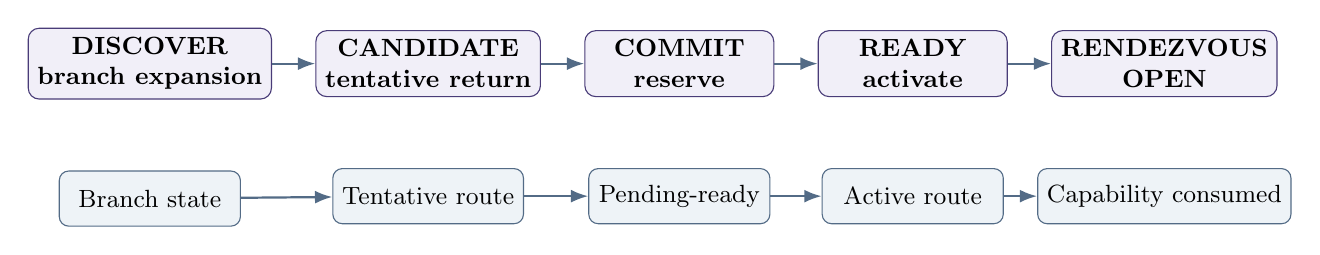
\begin{tikzpicture}[
  node distance=7mm and 5.5mm,
  box/.style={draw=accent,rounded corners=1.4mm,fill=softaccent,minimum height=8mm,minimum width=24mm,align=center,font=\small\bfseries},
  smallbox/.style={draw=accenttwo,rounded corners=1.2mm,fill=softblue,minimum height=7mm,minimum width=23mm,align=center,font=\small},
  arr/.style={-{Latex[length=2.2mm]},thick,color=accenttwo}
]
\node[box] (discover) {DISCOVER\\branch expansion};
\node[box,right=of discover] (candidate) {CANDIDATE\\tentative return};
\node[box,right=of candidate] (commit) {COMMIT\\reserve};
\node[box,right=of commit] (ready) {READY\\activate};
\node[box,right=of ready] (open) {RENDEZVOUS\\OPEN};
\draw[arr] (discover) -- (candidate);
\draw[arr] (candidate) -- (commit);
\draw[arr] (commit) -- (ready);
\draw[arr] (ready) -- (open);
\node[smallbox,below=9mm of discover] (branch) {Branch state};
\node[smallbox,below=9mm of candidate] (tentative) {Tentative route};
\node[smallbox,below=9mm of commit] (pending) {Pending-ready};
\node[smallbox,below=9mm of ready] (active) {Active route};
\node[smallbox,below=9mm of open] (redeemed) {Capability consumed};
\draw[arr] (branch) -- (tentative);
\draw[arr] (tentative) -- (pending);
\draw[arr] (pending) -- (active);
\draw[arr] (active) -- (redeemed);
\end{tikzpicture}
\caption{Protocol phases and principal state. Every state also has an independent expiry path.}
\label{fig:phases}
\end{figure}

\subsection{Local discovery state}

The initiator maintains an application request, private descriptor, expanding-ring schedule, cumulative budget, candidate set, and selection deadline. These values are local. The relay-visible object is a branch context bound to one ingress peer, one branch token, one incoming reply public key, one service-query nonce, finite expiry, and bounded child mappings.

The absence of a global attempt identifier prevents network-wide equality tests but also prevents perfect duplicate suppression when independently transformed branches converge. The resource model therefore treats each branch context as separately chargeable.

\section{Forward discovery and U1 transformation}
\label{sec:forward}

\subsection{Initiator behavior}

The initiator performs bounded expanding-ring discovery. The ring schedule, candidate threshold, retry policy, and cumulative budget remain local. For each selected first-hop peer, it creates an independent branch token $\beta_0$, reply key pair $(x_0,X_0)$, and service-query nonce $\nu_0$.

\begin{algorithm}[ht]
\caption{Initiator creates one first-hop branch}
\label{alg:initbranch}
\begin{algorithmic}[1]
\Require first-hop peer $p$, hop limit $d_{\max}$, local budget $\mathcal B$
\State $\beta_0\sample\{0,1\}^{128}\setminus\{0^{128}\}$
\State $x_0\sample\Zq\setminus\{0\}$; $X_0\gets x_0B$
\State $\nu_0\sample\{0,1\}^{256}\setminus\{0^{256}\}$
\State $m\gets\mathsf{Discover}(\beta_0,X_0,\nu_0,d_{\max},\mathcal B.\mathsf{propagation})$
\State $M\gets\Encode_{\Mtwo}(m,\code{0101})$
\State send $\mathsf{W2FragmentAndSeal}(p,M)$
\State record $(p,\beta_0,x_0,t_e)$ in local discovery state
\end{algorithmic}
\end{algorithm}

\subsection{Receive and validation order}

A relay processes input in the following order:

\begin{enumerate}
  \item parse the public \Wtwo{} link header;
  \item perform a non-mutating preliminary replay-window check;
  \item authenticate and decrypt the cell;
  \item advance replay state only after successful authentication;
  \item validate the encrypted fragment header and suite;
  \item reserve bounded reassembly resources;
  \item complete and canonically validate the fragment set;
  \item decode one \Mtwo{} message and verify suite agreement;
  \item apply per-peer and global admission limits;
  \item allocate branch or route-semantic state;
  \item execute the message-specific transition.
\end{enumerate}

This order prevents unauthenticated traffic from reserving a future sequence number or allocating route-semantic state.

\subsection{Per-child transformation}

For each admitted child, an honest relay creates a representation independent of both the incoming branch and its other children.

\begin{algorithm}[ht]
\caption{Relay forwards one admitted \Rone{} child branch}
\label{alg:forwardchild}
\begin{algorithmic}[1]
\Require decoded branch $(\beta_i,X_i,\nu_i,d)$ and child peer $c$
\State enforce branch, peer, node, cell, byte, work, and time limits
\State $\beta_{i+1}\sample\{0,1\}^{128}\setminus\{0^{128}\}$
\State $\delta_i\sample\Zq\setminus\{0\}$
\State $X_{i+1}\gets X_i+\delta_iB$
\State $\nu_{i+1}\sample\{0,1\}^{256}\setminus\{0^{256}\}$
\State store child mapping $(\beta_i,c,\beta_{i+1},\delta_i,X_i,X_{i+1},t_e)$
\State $m'\gets\mathsf{Discover}(\beta_{i+1},X_{i+1},\nu_{i+1},d-1,\ldots)$
\State $M'\gets\Encode_{\Mtwo}(m',\code{0101})$
\State $\mu'\sample\{0,1\}^{128}\setminus\{0^{128}\}$
\State fragment $M'$ canonically and emit fresh \Wtwo{} cells to $c$
\end{algorithmic}
\end{algorithm}

\subsection{Loops and convergence}

A relay rejects exact reuse of a live ingress token from the same peer and link epoch. It does not assume that two different tokens identify different logical discoveries. Immediate edge reversal is prohibited, and a relay MAY use bounded adjacent-local loop hints that do not cross a link boundary. Every accepted context is independently limited and expires locally.

\begin{proposition}[No explicit cross-hop equality handle]
In the active \Rone{} forward transform, the outgoing branch token, service nonce, reply public key, logical-message bytes, local wire message identifier, padding, AEAD nonce, and ciphertext differ from the incoming representation except with negligible collision probability.
\end{proposition}

\begin{proof}
Tokens, nonces, message identifiers, padding, and link nonces are freshly sampled. The reply key is additively changed by a non-zero random scalar. The logical message is reconstructed and fragmented under a new local identifier. Adjacent-link ciphertext is produced under the outgoing link key. The only intentionally preserved values are bounded semantic controls such as remaining hop limit and profile identifiers.
\end{proof}

\section{Candidate return and route activation}
\label{sec:reverse}

\subsection{Gateway candidate}

A gateway that admits the branch constructs
\begin{equation}
P_G=(\pi_G,t_{\mathrm{offer}},X_d,c_G,n_G,\mathsf{params}),
\label{eq:candidatepayload}
\end{equation}
where $c_G$ is a commit challenge and $n_G$ is a fresh nonce. It signs the domain-separated transcript with its descriptor-authenticated Ed25519 key and seals the result to $X_d$ using the retained reply KEM.

The gateway pseudonym is protected inside the sealed payload. Relays learn only that a candidate is returning on a live branch.

\subsection{Nested reverse layers}

At relay $n_i$, the reverse layer contains the stored tweak, adjacent route labels, child candidate token, expiry, and child capsule:
\begin{equation}
L_i=(\delta_i,\lambda_i^{\rightarrow},\lambda_i^{\leftarrow},
\gamma_i,t_e,C_{i+1}).
\end{equation}
The relay seals $L_i$ to $X_i$ and forwards the resulting capsule to its parent under a fresh reverse token.

\subsection{Initiator opening}

Starting with $x_0$, the initiator opens the outer layer, obtains $\delta_0$, derives $x_1=x_0+\delta_0\bmod q$, and repeats until it reaches the gateway payload.

\begin{algorithm}[ht]
\caption{Initiator validates one nested candidate}
\label{alg:opencandidate}
\begin{algorithmic}[1]
\Require root reply secret $x_0$, capsule $C_0$, private descriptor $\mathsf{RDesc}$
\State $x\gets x_0$; $C\gets C_0$; $\mathsf{path}\gets[\ ]$
\Loop
  \State $P\gets\Open_{\mathsf{TRKEM}}(x,C,\mathsf{context})$
  \If{$P$ is a relay layer $(\delta,\lambda^{\rightarrow},\lambda^{\leftarrow},\gamma,t_e,C')$}
    \State reject if expired or non-canonical
    \State append local route material to $\mathsf{path}$
    \State $x\gets x+\delta\bmod q$; $C\gets C'$
  \ElsIf{$P$ is a signed gateway payload}
    \State verify transcript, descriptor key, offer deadline, and final reply key
    \State reject unless $P.\pi_G\in\mathsf{RDesc}.\mathsf{acceptable\_gateways}$
    \State \Return validated candidate and $\mathsf{path}$
  \Else
    \State \Return $\bot$
  \EndIf
\EndLoop
\end{algorithmic}
\end{algorithm}

\subsection{Commit and readiness}

Candidate return creates only tentative route mappings. The initiator selects one candidate and sends \textsc{Commit} using the first forward route label. Each relay verifies the expected parent label and challenge, reserves bounded capacity, moves the selected mapping to \code{PENDING\_READY}, and forwards under the next local label. The gateway returns \textsc{Ready}; each relay authenticates the reverse transition and moves the mapping to \code{ACTIVE}.

Application data and \textsc{Rendezvous-Open} MUST NOT be forwarded before the initiator authenticates final \textsc{Ready}. This separates discovery success from route authorization.

\section{E1 event lifecycle}
\label{sec:lifecycle}

\subsection{Half-open deadlines}

Every state created at $t_c$ with expiry $t_e$ is valid only on
\begin{equation}
[t_c,t_e)=\{t\mid t_c\le t<t_e\}.
\end{equation}
An event at exactly $t_e$ observes the state as expired. Timer rescheduling may extend a state only through an explicit transition; an older timer cannot shorten a later deadline.

\subsection{Equal-time precedence}

When events share one timestamp, an implementation applies this order:

\begin{enumerate}
  \item authenticated cell receipt and completion of already admitted reassembly;
  \item message-specific transition whose preconditions were valid immediately before the timestamp;
  \item local cancellation or selection decision;
  \item expiry and resource reclamation;
  \item advisory outbound cleanup.
\end{enumerate}

This order is deterministic but does not guarantee delivery. A candidate received after the local candidate window is closed is rejected even if remote branch state remains live.

\subsection{State progression}

\begin{table}[ht]
\centering
\caption{Principal relay-state transitions}
\label{tab:states}
\begin{tabularx}{\textwidth}{@{}p{0.19\textwidth}p{0.23\textwidth}p{0.23\textwidth}X@{}}
\toprule
Current state & Event & Next state & Effect \\
\midrule
None & valid \textsc{Discover} & Branch & Store parent/child branch mappings and expiry. \\
Branch & valid \textsc{Candidate} & Tentative & Store local route labels; branch may remain for other children. \\
Tentative & selected \textsc{Commit} & Pending-ready & Reserve capacity and forward commit. \\
Pending-ready & valid \textsc{Ready} & Active & Authorize route forwarding. \\
Any live state & expiry & None & Reclaim locally; optional advisory cleanup. \\
Tentative/pending & \textsc{Cancel}/\textsc{Abort} & None & Best-effort early cleanup. \\
Active & \textsc{Close} or expiry & None & Reclaim active mapping. \\
\bottomrule
\end{tabularx}
\end{table}

Delayed candidates from earlier expanding rings MAY be accepted while the same logical candidate window remains open. They do not reopen a closed window and do not expand the cumulative budget.

\section{M2 logical messages and W2 wire cells}
\label{sec:messages}

\subsection{Layer separation}

A logical protocol message and an observable transmission unit solve different problems. \Mtwo{} therefore defines a compact canonical message, while \Wtwo{} defines fixed-size cells. A short message normally occupies one cell; a deeply nested candidate may occupy several. This removes the former artificial route-depth limit caused by requiring every logical message to fit in one record.

\subsection{M2 envelope}

Every \Mtwo{} message has the canonical form
\begin{equation}
M=\mathsf{version}\concat\mathsf{type}\concat\mathsf{suite}
\concat\mathsf{body\_length}\concat\mathsf{body}.
\label{eq:m2}
\end{equation}
Version, type, and suite are fixed width. Variable lengths use minimal unsigned base-128 LEB128. A decoder rejects overlong encodings, unterminated values, trailing bytes, inconsistent nested lengths, and suite-specific field lengths outside their bounds.

The active suite identifier is \code{0101}. In an \Rone{} \textsc{Discover}, the suite-specific field is exactly 32 bytes and contains $\nu_i$. The raw capability $\tau$, its hash, gateway pseudonym, endpoint handle, and destination authentication material are prohibited from this message class.

\subsection{W2 cell}

A \Wtwo{} record has length
\begin{equation}
L_C=12+1024+16=1052\ \text{bytes}.
\end{equation}
The 12-byte public header contains a directional link epoch and sequence number. The encrypted 1,024-byte plaintext contains a 32-byte fragment header, up to 992 message bytes, and fresh random padding. ChaCha20-Poly1305 contributes the 16-byte authentication tag~\cite{chacha}.

The encrypted fragment header contains the local message identifier $\mu$, suite, fragment index, fragment count, total logical length, and current fragment length. It is authenticated together with the public link header as associated data.

\subsection{Canonical fragmentation}

For a logical message of length $L$,
\begin{equation}
q(M)=\left\lceil\frac{L}{992}\right\rceil,
\qquad 1\le L\le16{,}384,
\qquad 1\le q(M)\le17.
\label{eq:fragmentcount}
\end{equation}
Every non-final fragment contains exactly 992 message bytes. The final fragment contains the remainder. Alternative short-fragment decompositions are invalid.

\subsection{Bounded reassembly}

A context is keyed by authenticated directional link scope and local message identifier. It reserves the declared total logical length, accepts out-of-order fragments, treats exact duplicates idempotently, invalidates the whole context on conflicting duplicate bytes or metadata, and expires after a finite deadline.

\begin{algorithm}[ht]
\caption{Bounded \Wtwo{} receive pipeline}
\label{alg:reassembly}
\begin{algorithmic}[1]
\Require cell record $w$ from authenticated peer scope $\ell$
\State parse public epoch and sequence; perform non-mutating replay precheck
\State authenticate and decrypt $w$; on failure return generic reject
\State advance replay state
\State decode and validate fragment header $f$
\State reject if suite disabled, lengths non-canonical, or bounds exceeded
\State obtain or allocate bounded context $R[\ell,f.\mu]$
\State reject and invalidate context on metadata conflict
\State store fragment or accept exact duplicate idempotently
\If{all canonical fragments are present}
  \State concatenate exactly $f.L$ bytes and delete reassembly context
  \State decode one canonical \Mtwo{} message
  \State require \Mtwo{}/\Wtwo{} suite agreement
  \State only now invoke route-semantic processing
\EndIf
\end{algorithmic}
\end{algorithm}

\begin{property}[No route state before complete decoding]
A partial, unauthenticated, non-canonical, or cross-suite fragment set cannot allocate branch, candidate, tentative, pending, or active route state.
\end{property}

\section{Retained cryptographic components}
\label{sec:crypto}

\subsection{Reply-key transformation}

For one branch, the initiator samples $x_0\in\Zq\setminus\{0\}$ and publishes $X_0=x_0B$. Relay $i$ samples $\delta_i\in\Zq\setminus\{0\}$ and computes
\begin{equation}
X_{i+1}=X_i+\delta_iB.
\label{eq:tweak}
\end{equation}
The initiator later reconstructs
\begin{equation}
x_{i+1}=x_i+\delta_i\pmod q.
\label{eq:tweaksecret}
\end{equation}

\begin{proposition}[Tweak consistency]
If $X_i=x_iB$, then the public and secret transformations in \cref{eq:tweak,eq:tweaksecret} satisfy $X_{i+1}=x_{i+1}B$.
\end{proposition}

\begin{proof}
By distributivity in the prime-order group,
$(x_i+\delta_i)B=x_iB+\delta_iB=X_i+\delta_iB$.
\end{proof}

Each first-hop branch uses an independent root key. Relays reject the identity encoding and non-canonical points according to RFC~9496~\cite{ristretto}.

\subsection{Reply KEM and nested encryption}

The reply construction is HPKE-inspired: it combines ephemeral group agreement, domain-separated HKDF-SHA-256, and ChaCha20-Poly1305~\cite{hpke,hkdf,chacha}. It is not RFC~9180 HPKE because the public key is deliberately tweakable and no registered HPKE KEM provides the same interface. Context binds protocol version, message class, suite, direction, route stage, and the exact public keys used.

Fresh encapsulation randomness and AEAD nonce are required for every layer. Decryption, point-validation, transcript, and authentication failures map to one externally visible rejection class.

\subsection{Gateway authentication}

The signed candidate transcript includes, in fixed order, the protocol domain, version, suite, gateway pseudonym, offer deadline, final reply public key, commit challenge, candidate nonce, and selected parameter digest. Ed25519 verification follows RFC~8032~\cite{eddsa}. The descriptor must bind the verification key to the accepted short-lived pseudonym.

\subsection{Adjacent-link protection}

Link keys are distinct from reply and signing keys. Each directional link epoch provides unique nonces or sequence-derived nonce material. The replay window advances only after successful AEAD verification, preventing unauthenticated input from reserving future sequence numbers.

\section{Research cryptographic profiles and citations}
\label{sec:researchcrypto}

\subsection{C1 negative control}

The repository retains a GJJS-style universal-re-encryption capsule as a negative control~\cite{gjjs}. Its components can be rerandomized without a recipient key, but a compromised relay can multiply selected components by a related factor. The ratio between those components survives the honest rerandomization relation and is recognizable by a colluding downstream relay. This experiment demonstrates why byte-level freshness and passive rerandomization correctness do not imply resistance to active cross-hop tags, consistent with the stronger security distinctions discussed by Banfi, Maurer, and Ritsch~\cite{ure2023}.

C1 is not network enabled and MUST NOT be cited as evidence for active unlinkability.

\subsection{Receiver-anonymous rerandomizable RCCA target}

Wang et al. define receiver-anonymous rerandomizable RCCA-secure public-key encryption and give a generic construction based on rerandomizable tag smooth-projective hash functions~\cite{anonrcca2021}. Their result is directly relevant to an endpoint-specific discovery ciphertext because the desired transform must preserve both plaintext and recipient while hiding the recipient and resisting non-replay modifications.

The protocol-facing security target was expressed independently as correctness, message confidentiality, receiver anonymity, public ciphertext-only rerandomization, transformed-ciphertext unlinkability, replay-equivalence handling, active-tag resistance, canonical encoding, and composition with the relay transform. The application-level URE treatment of Banfi et al. motivates separating these properties rather than relying on one syntactic rerandomization equation~\cite{ure2023}.

\subsection{Concrete k=2 audit}

A deterministic transcription implements the cited paper's $k=2$ key generation, encryption, decryption, canonical encoding, mutation rejection, and linear strand equations~\cite{anonrcca2021}. The literal finite-field interpretation uses the map
\begin{equation}
\mu(u)=u\bmod q
\end{equation}
from a quadratic-residue group modulo $p=2q+1$ into the field modulo $q$.

\begin{proposition}[Literal reduction is not generally multiplicative]
Under ordinary multiplication in $\operatorname{QR}^{*}_{p}$, the map $\mu(u)=u\bmod q$ is not a group homomorphism in general.
\end{proposition}

\begin{proof}
For the valid small chain $q=5$, $p=11$, and $r=23$, choose $u=3$ and $v=4$, both in $\operatorname{QR}^{*}_{11}$. Then $uv\bmod p=1$, hence $\mu(uv\bmod p)=1$, while
$\mu(u)\mu(v)\bmod q=3\cdot4\bmod5=2$.
\end{proof}

An exhaustive checker repeats this test over every admissible pair in several small Cunningham chains and finds a counterexample in every nontrivial chain examined. This is a narrow audit of the literal implementation path. It does not refute the paper's generic framework, an unrecorded embedding, or an author-confirmed correction. The corresponding suite identifier remains disabled and every network operation fails closed.

\subsection{Updatable and randomizable PKE}

Dowling et al. define updatable and randomizable signatures and public-key encryption for strongly anonymous ratcheted key exchange~\cite{urpke2022}. Their randomization operation transforms an encryption key and ciphertext together. The earlier \ProtoName{} endpoint-specific design required a relay that knows neither recipient key nor secret to transform only the ciphertext while preserving the same recipient. The interfaces are therefore different, and the cited construction is not enabled as an eligibility suite.

\subsection{Gate decision}

Because no reviewed concrete endpoint-specific primitive currently satisfies the complete protocol interface, the active design adopts \Rone{}. This is a security-engineering decision rather than a claim that rendezvous capabilities dominate receiver-anonymous rerandomizable encryption. It trades a difficult cryptographic dependency for a directory-and-gateway trust boundary that can be specified, measured, and replaced independently.

\section{Security analysis}
\label{sec:security}

\subsection{Endpoint material absent from discovery}

The active \textsc{Discover} grammar contains no $\tau$, $h_\tau$, destination address, destination key, gateway pseudonym, or endpoint handle. The suite-specific field is the random non-semantic nonce $\nu_i$. A byte-search conformance test verifies that an issued capability does not occur in the encoded discovery message.

This property is stronger than merely encrypting a destination selector against passive observation: compromised ordinary relays also receive no endpoint-specific selector from the protocol. They may still infer destination information from topology, timing, gateway choice, or external knowledge.

\subsection{Per-hop replacement argument}

At an honest relay, all adjacent capabilities and wire representations are replaced. The reply key is algebraically related because the initiator must reconstruct it, but the public point changes by an independently sampled group element. A passive downstream relay lacks the prior point unless it colludes with an upstream relay. The active protocol makes no claim that the custom reply-key relation alone resists every malicious algebraic tag; candidate authentication and failure normalization limit accepted modifications, while the explicit active-tag experiment focuses on the discovery field.

\subsection{Capability confidentiality and replay}

The capability is absent from discovery and candidate traffic. It is sent only after \textsc{Ready} inside end-to-end route protection. Atomic commitment lookup and deletion enforce at most one successful redemption. This does not protect a capability stolen from an initiator before first use; the attacker may race the legitimate user. A production descriptor profile should bind redemption to an authenticated client handshake and use short expiries.

\subsection{Gateway and directory exposure}

A gateway learns the registration commitment and observes successful redemption. The directory learns which descriptor it delivers unless private information retrieval, oblivious access, replication, or another privacy mechanism is specified. The active protocol therefore provides no unlinkability guarantee against directory--gateway collusion. Multiple gateways, short-lived pseudonyms, descriptor rotation, and separated operators may reduce exposure but are not proofs.

\subsection{Cell-length and fragmentation leakage}

Fixed cell length prevents exact per-cell length classification. Multi-cell messages still reveal a fragment burst unless scheduling hides it. A candidate's cell count can correlate with reverse-layer depth. \Wtwo{} therefore supports but does not itself provide message-count or timing privacy.

\subsection{Failure normalization}

Malformed capability, wrong gateway, expiry, replay, signature failure, nested decryption failure, disabled suite, cross-suite fragment, non-canonical message, and invalid route label all map to a generic protocol rejection at their observation boundary. Implementations must also normalize timing and logging sufficiently to avoid turning internal diagnostics into an oracle.

\section{Resource and denial-of-service model}
\label{sec:resources}

\subsection{Why privacy consumes state}

A stable attempt identifier allows broad duplicate suppression but creates a correlation handle. \Uone{} removes that handle, so converging branches may allocate separate contexts. The protocol therefore treats resource bounds as normative security properties rather than implementation suggestions.

\subsection{Required bounds}

An implementation MUST define finite limits for:

\begin{itemize}
  \item authenticated cells per peer, direction, and time window;
  \item concurrent reassembly contexts and aggregate reserved bytes;
  \item message length, fragment count, and reassembly duration;
  \item branch contexts per ingress peer, per node, and globally;
  \item fan-out, hop limit, expanding-ring attempts, and cumulative transmissions;
  \item candidate, tentative, pending-ready, and active route mappings;
  \item cryptographic operations and queue entries;
  \item gateway registration records, failed redemptions, and endpoint-handle lifetime;
  \item logical discovery time and all state deadlines.
\end{itemize}

\subsection{Admission order}

Cheap syntactic and authenticated-link checks precede expensive group, signature, or nested-decryption operations. Per-peer token buckets limit fresh-branch creation. Global and per-node caps remain necessary because an adversary can distribute traffic across peers. A failed stage does not consume resources reserved for later stages.

\subsection{Amplification}

Let $f$ be fan-out, $d$ hop limit, and $a_i$ the fraction of branches admitted at depth $i$. An upper bound on forward branch transmissions is
\begin{equation}
T\le \sum_{i=1}^{d} f^i\prod_{j=1}^{i}a_j.
\label{eq:amplification}
\end{equation}
This bound ignores convergence and early responder termination, but shows why broad fixed flooding is unsuitable. Expanding rings and cumulative budgets reduce expected cost when gateways are sufficiently dense.

\section{Deterministic evaluation}
\label{sec:evaluation}

\subsection{Method and scope}

The repository contains deterministic event models and exact conformance vectors. The results are regression and falsification evidence, not production benchmarks, cryptographic proofs, or measurements of a deployed network. Each scenario fixes seeds, topology parameters, timers, budgets, and attacker actions.

\subsection{Expanding-ring discovery}

On 500-node random graphs with average degree eight and 100 runs per responder density, expanding rings reduced transmissions relative to a fixed broad flood while retaining high discovery success. At two percent responder density, success was 100 percent and mean transmissions fell from 895.12 to 157.65, an 82.39 percent reduction. State allocations fell by 72.28 percent. These figures justify an expanding-ring default, not a universal parameter choice.

\subsection{U1 state cost}

Removing a stable identifier increases branch-context state because converging branches cannot be globally merged. With hop limit four and fan-out three, the model observed an 85 percent success rate, 118.34 mean transmissions, and 15.60 percent state overhead relative to the identifier-bearing control. With hop limit five and fan-out four, 91 percent of runs exhausted the configured budget. Privacy and scalability therefore depend on conservative fan-out and strict cumulative limits.

\subsection{Lifecycle and attack admission}

The event-driven model evaluates delayed candidates, loss, duplication, cancellation, and fresh-branch attack traffic. In the fresh-branch attack scenario, a per-ingress token bucket increased route success from 32 to 76 percent and reduced mean total transmissions from 1,440.33 to 1,176.56. Every evaluated run reclaimed all route state.

\subsection{Message and cell capacity}

A six-layer candidate encoded to 909 logical bytes and fit in one cell. Seven layers encoded to 1,024 bytes and required two cells. Twelve layers required 1,599 bytes and two cells; sixteen layers required 2,059 bytes and three cells. Variable-length messages over fixed cells therefore remove the single-record route-depth limit.

Under independent two percent cell loss and no retransmission, clean route success decreased with hop count: 80 percent at two hops, 65 percent at five, 50 percent at eight, and 30 percent at twelve. This result identifies bounded reliability as a required later profile.

\subsection{R1 and cryptographic controls}

\begin{table}[ht]
\centering
\caption{R1 active-tag comparison, 100 deterministic runs per scenario}
\label{tab:r1results}
\begin{tabularx}{\textwidth}{@{}p{0.33\textwidth}rrrrX@{}}
\toprule
Scenario & Success & Mean tx & Mean bytes & Crypto failures & Downstream tag observations \\
\midrule
R1 clean & 1.00 & 16 & 16,832 & 0 & 0 \\
R1 literal nonce marker & 1.00 & 16 & 16,832 & 0 & 0 \\
C1 ratio-tag negative control & 0.00 & 8 & 8,416 & 1 & 1 \\
Symbolic C2 marker control & 0.00 & 4 & 4,208 & 1 & 0 \\
\bottomrule
\end{tabularx}
\end{table}

The \Rone{} marker is erased by honest replacement, so the downstream colluder receives no recognizable descendant. This test covers only a literal field marker under the modeled transform. It does not establish traffic-flow unlinkability or security against tagging through delays, selective forwarding, topology, or other fields. The C1 row remains a known-failing control, while the symbolic C2 row tests failure placement rather than cryptography.

\subsection{Capability conformance}

Tests establish that the raw capability does not occur in encoded \textsc{Discover} bytes; every relay replacement changes the query nonce; the correct gateway redeems once; replay, expiry, wrong gateway, duplicate registration, and the all-zero token fail; and failed redemption does not preserve a live record beyond the defined deadline. A tracked deterministic vector set binds the suite identifier, service-class label, three successive nonce replacements, capability commitment, gateway-local registry hash, successful first redemption, and rejected wrong-gateway, replay, and expiry cases.

\section{Limitations and open problems}
\label{sec:limitations}

\subsection{Private descriptor distribution}

The largest new dependency is $Q$. A complete deployment needs a private lookup and descriptor distribution protocol. Possible mechanisms include replicated encrypted descriptors, authenticated access control, oblivious or private information retrieval, and gateway/operator separation. None is selected here.

\subsection{Gateway correlation}

A gateway can correlate registration time, redemption time, endpoint handle, and route-local observations. Multiple gateways and short epochs limit concentration but do not remove this visibility. A gateway may also selectively refuse service or create distinguishing delays.

\subsection{Reliability and scheduling}

\Wtwo{} fragmentation requires bounded retransmission, acknowledgement, or erasure recovery. Retransmissions must use fresh link encryption and must not create a stable cross-hop identifier. A traffic scheduler must define interleaving, batch size, release distribution, count padding, chaff, and behavior under congestion. Until then, timing and fragment-count correlations remain outside the claim.

\subsection{Reply-key analysis}

The additive reply-key transform and custom KEM require an independent analysis for related-key behavior, malicious point selection, active tagging, transcript substitution, and side channels. Standard components do not automatically prove security of their composition.

\subsection{Post-quantum migration}

The active reply, signature, and link profiles are classical. Cryptographic agility is encoded, but a post-quantum suite must define exact key sizes, candidate expansion, cell impact, and transition rules. Merely adding an identifier is not a migration strategy.

\subsection{Network economics and policy}

The protocol does not define transit incentives, inter-domain policy, Sybil resistance, gateway admission, reputation, or abuse adjudication. These concerns can dominate deployment viability even when the control-plane mechanics are sound.

\section{Implementation and review strategy}
\label{sec:implementation}

A staged implementation should preserve module boundaries:

\begin{enumerate}
  \item independent \Mtwo{} and \Wtwo{} codec implementations with differential tests and fuzzing;
  \item a typed eligibility-provider boundary containing active \Rone{} and research-only controls;
  \item a deterministic \Eone{} state machine separated from transport I/O;
  \item constant-time or timing-normalized cryptographic failure paths;
  \item a persistent, atomic gateway capability store with concurrency tests;
  \item an independent implementation of the reply KEM and candidate transcript;
  \item a reliability profile for multi-cell messages;
  \item a scheduler and traffic-correlation experiment;
  \item external cryptographic and protocol review before any production claim.
\end{enumerate}

The disabled C2 transcription should remain reproducible. An author query should identify the exact equation, parameter chain, interpretation, counterexample, and executable checker, and ask whether an omitted embedding, different group action, or erratum resolves the discrepancy. A correction may reopen an endpoint-specific suite, but must not silently change the active \Rone{} security model.

\section{Conclusion}
\label{sec:conclusion}

\ProtoName{} defines bounded route discovery with no transmitted source route or network-wide discovery identifier. The current protocol removes endpoint-specific material from forward exploration, discovers generic rendezvous gateways, authenticates candidates through nested reverse encryption, activates one selected route through \textsc{Commit} and \textsc{Ready}, and presents a single-use capability only after activation.

The message and wire layers are separated: logical messages remain canonical and variable length, while every adjacent-link cell has fixed length and bounded reassembly. Route and reassembly state have explicit lifetimes and budgets. The security claims distinguish per-hop representation replacement from traffic-flow anonymity and expose the directory/gateway trust boundary introduced by the rendezvous design.

This revision resolves the active-protocol dependency on an unimplemented universal-rerandomization primitive without discarding the associated research. The failed C1 and C2 candidates remain cited, executable, and falsifiable. The resulting document is a coherent interoperability and review baseline, not a production-ready anonymity guarantee.

\appendix
\section{Normative requirement summary}
\label{app:normative}

The keywords ``MUST'', ``MUST NOT'', ``REQUIRED'', ``SHOULD'', ``SHOULD NOT'', and ``MAY'' are interpreted according to BCP~14~\cite{rfc2119,rfc8174}.

An implementation claiming \Uone{}, \Eone{}, \Rone{}, \Mtwo{}, and \Wtwo{} conformance MUST:

\begin{enumerate}
  \item omit endpoint capabilities, endpoint keys, endpoint addresses, descriptor commitments, gateway pseudonyms, global discovery identifiers, and complete routes from \textsc{Discover};
  \item encode the active suite as \code{0101} and require exactly one non-zero 32-byte service-query nonce;
  \item replace branch token, query nonce, reply public key, logical-message encoding, wire message identifier, padding, and link ciphertext for every forwarded child;
  \item use an independent root reply key for every first-hop branch;
  \item verify the gateway pseudonym only inside the authenticated candidate payload and only against the private descriptor;
  \item create tentative state on \textsc{Candidate}, reserve pending state on \textsc{Commit}, and authorize data only after final \textsc{Ready};
  \item transmit the rendezvous capability only inside an end-to-end protected active route;
  \item store only the domain-separated capability commitment at a gateway and atomically delete the record on successful redemption;
  \item reject replay, expiry, wrong gateway, all-zero capability, duplicate live registration, and malformed request through one generic failure class;
  \item encode each logical operation as one canonical \Mtwo{} message with no semantic padding or trailing bytes;
  \item enforce $1\le|M|\le16{,}384$ and canonical fragmentation into at most 17 \Wtwo{} cells;
  \item encode every \Wtwo{} record as exactly 1,052 bytes and advance replay state only after adjacent-link authentication;
  \item accept out-of-order fragments, process exact duplicates idempotently, invalidate conflicting duplicates, and bound contexts, bytes, fragments, and time;
  \item allocate no route-semantic state before complete reassembly, suite agreement, and canonical message decoding;
  \item enforce finite per-peer and global limits for cells, branches, candidates, routes, queues, cryptographic work, registrations, redemption failures, and setup time;
  \item use half-open state lifetimes and the \Eone{} equal-time precedence order;
  \item map disabled suite, cryptographic, message, cell, reassembly, route, and redemption failures to externally normalized rejection behavior;
  \item keep C1, symbolic C2, and the C2-$k=2$ transcription disabled for operational network selection;
  \item make batch-local unlinkability claims only for a declared scheduler and anonymity-set treatment;
  \item refrain from private-directory, directory/gateway-collusion, traffic-flow, post-quantum, or production-security claims unless separately specified and reviewed.
\end{enumerate}

\section{Message-class summary}
\label{app:messages}

\begin{table}[ht]
\centering
\caption{Logical control operations}
\label{tab:messageclasses}
\begin{tabularx}{\textwidth}{@{}p{0.19\textwidth}p{0.20\textwidth}X@{}}
\toprule
Operation & Direction & Principal purpose \\
\midrule
\textsc{Discover} & outward & Create branch state; carries token, reply key, non-semantic query nonce, and bounded propagation controls. \\
\textsc{Candidate} & inward & Return nested authenticated gateway offer and install tentative route labels. \\
\textsc{Commit} & outward & Select one candidate, prove commit challenge, and reserve route capacity. \\
\textsc{Ready} & inward & Confirm gateway activation and authorize route use. \\
\textsc{Rendezvous-Open} & outward over active route & Redeem one-time endpoint capability and start local gateway rendezvous. \\
\textsc{Cancel} & outward/inward advisory & Reclaim unselected tentative state early. \\
\textsc{Abort} & either direction advisory & Reclaim failed pending state early. \\
\textsc{Close} & either direction advisory & Reclaim active route early. \\
\textsc{Chaff} & scheduler-defined & Occupy a fixed cell without route-semantic content. \\
\bottomrule
\end{tabularx}
\end{table}

\section{Research-provider status}
\label{app:providers}

\begin{table}[ht]
\centering
\caption{Eligibility-provider boundary}
\label{tab:providers}
\begin{tabularx}{\textwidth}{@{}p{0.26\textwidth}p{0.14\textwidth}p{0.20\textwidth}X@{}}
\toprule
Provider & Suite & Network status & Purpose \\
\midrule
R1 rendezvous capability & \code{0101} & Active experimental & Generic gateway discovery; endpoint capability after \textsc{Ready}. \\
C1 URE negative control & \code{0001} & Research only & Reproduce persistent algebraic ratio tagging. \\
C2 symbolic oracle & \code{0002} & Research only & Exercise ideal replay-equivalence and mutation-rejection placement. \\
C2 $k=2$ transcription & \code{7f02} & Disabled & Reproduce source equations and finite-field audit; fail closed. \\
\bottomrule
\end{tabularx}
\end{table}

\section{Canonical encoding note}

\Mtwo{} uses minimal unsigned base-128 LEB128 for variable lengths. Every decoder rejects a longer encoding, an unterminated value, a value above its field limit, trailing bytes, or a nested length exceeding its container. Fixed-width numeric fields are unsigned big-endian values.

\Wtwo{} uses fixed-width unsigned big-endian integers in the public 12-byte header and encrypted 32-byte fragment header. The suite identifier in every fragment must agree with the completed \Mtwo{} message. Every non-final fragment contains exactly 992 message bytes and the final fragment exactly the remainder. The 1,052-byte record length hides exact per-cell content length, but not cell count, direction, or timing.

\begingroup
\small
\begin{thebibliography}{99}
\setlength{\itemsep}{0.2\baselineskip}

\bibitem{rfc2119}
S. Bradner,
``Key words for use in RFCs to Indicate Requirement Levels,''
BCP 14, RFC 2119, March 1997.

\bibitem{rfc8174}
B. Leiba,
``Ambiguity of Uppercase vs Lowercase in RFC 2119 Key Words,''
BCP 14, RFC 8174, May 2017.

\bibitem{sphinx}
G. Danezis and I. Goldberg,
``Sphinx: A Compact and Provably Secure Mix Format,''
in \emph{IEEE Symposium on Security and Privacy}, 2009, pp. 269--282.

\bibitem{hornet}
C. Chen, D. E. Asoni, D. Barrera, G. Danezis, and A. Perrig,
``HORNET: High-speed Onion Routing at the Network Layer,''
in \emph{22nd ACM Conference on Computer and Communications Security}, 2015, pp. 1441--1454.

\bibitem{loopix}
A. M. Piotrowska, J. Hayes, T. Elahi, S. Meiser, and G. Danezis,
``The Loopix Anonymity System,''
in \emph{26th USENIX Security Symposium}, 2017, pp. 1199--1216.

\bibitem{taranet}
C. Chen, D. E. Asoni, A. Perrig, D. Barrera, G. Danezis, and C. Troncoso,
``TARANET: Traffic-Analysis Resistant Anonymity at the Network Layer,''
in \emph{IEEE European Symposium on Security and Privacy}, 2018, pp. 137--152.

\bibitem{gjjs}
P. Golle, M. Jakobsson, A. Juels, and P. Syverson,
``Universal Re-encryption for Mixnets,''
in \emph{Topics in Cryptology -- CT-RSA 2004}, LNCS 2964, 2004, pp. 163--178.

\bibitem{rcca2003}
R. Canetti, H. Krawczyk, and J. B. Nielsen,
``Relaxing Chosen-Ciphertext Security,''
in \emph{Advances in Cryptology -- CRYPTO 2003}, LNCS 2729, 2003, pp. 565--582.

\bibitem{keyprivacy2001}
M. Bellare, A. Boldyreva, A. Desai, and D. Pointcheval,
``Key-Privacy in Public-Key Encryption,''
in \emph{Advances in Cryptology -- ASIACRYPT 2001}, LNCS 2248, 2001, pp. 566--582,
doi:10.1007/3-540-45682-1\_33.

\bibitem{rcca2007}
M. Prabhakaran and M. Rosulek,
``Rerandomizable RCCA Encryption,''
in \emph{Advances in Cryptology -- CRYPTO 2007}, LNCS 4622, 2007, pp. 517--534.

\bibitem{anonrcca2021}
Y. Wang, R. Chen, G. Yang, X. Huang, B. Wang, and M. Yung,
``Receiver-Anonymity in Rerandomizable RCCA-Secure Cryptosystems Resolved,''
in \emph{Advances in Cryptology -- CRYPTO 2021}, LNCS 12828, 2021, pp. 270--300,
doi:10.1007/978-3-030-84259-8\_10; full version, IACR ePrint 2021/862.

\bibitem{ure2023}
F. Banfi, U. Maurer, and S. Ritsch,
``On the Security of Universal Re-Encryption,''
Cryptology ePrint Archive, Paper 2023/1165, 2023.

\bibitem{urpke2022}
B. Dowling, E. Hauck, D. Riepel, and P. R\"osler,
``Strongly Anonymous Ratcheted Key Exchange,''
in \emph{Advances in Cryptology -- ASIACRYPT 2022}; full version, IACR ePrint 2022/1187.

\bibitem{toroverview}
The Tor Project,
``Tor Rendezvous Specification, Version 3: Protocol Overview,''
Tor Specifications, section 13.2, accessed July 2026.

\bibitem{torintro}
The Tor Project,
``Tor Rendezvous Specification, Version 3: The Introduction Protocol,''
Tor Specifications, section 13.4, accessed July 2026.

\bibitem{torrendezvous}
The Tor Project,
``Tor Rendezvous Specification, Version 3: The Rendezvous Protocol,''
Tor Specifications, section 13.5, accessed July 2026.

\bibitem{hpke}
R. Barnes, K. Bhargavan, B. Lipp, and C. A. Wood,
``Hybrid Public Key Encryption,''
RFC 9180, February 2022.

\bibitem{ristretto}
H. de Valence, J. Grigg, M. Hamburg, I. Lovecruft, G. Tankersley, and F. Valsorda,
``The ristretto255 and decaf448 Groups,''
RFC 9496, December 2023.

\bibitem{hkdf}
H. Krawczyk and P. Eronen,
``HMAC-based Extract-and-Expand Key Derivation Function (HKDF),''
RFC 5869, May 2010.

\bibitem{chacha}
Y. Nir and A. Langley,
``ChaCha20 and Poly1305 for IETF Protocols,''
RFC 8439, June 2018.

\bibitem{eddsa}
S. Josefsson and I. Liusvaara,
``Edwards-Curve Digital Signature Algorithm (EdDSA),''
RFC 8032, January 2017.

\end{thebibliography}
\endgroup

\end{document}
